% AUTO-GENERATED durch diagram_generator (REV 7.6, TikZ-Heatmap)
\begin{figure}[!htbp]
\centering
\begin{tikzpicture}
\begin{axis}[
    width=0.9500\textwidth,
    height=0.4000\textheight,
    scale only axis,
    title={Heatmap: Lookup-Latenz p50 (ns/op) (Suchalgorithmus x Workload)},
    xlabel={Workload},
    ylabel={Suchalgorithmus},
    grid=both,
    enlargelimits=0.05,
    view={0}{90},
    colorbar,
    colormap/viridis,
    mesh/cols=21,
    xtick={0,1,...,20},
    ytick={0,1,...,3},
    xticklabels={coco\_p04\_neg0,coco\_p04\_neg100,coco\_p04\_neg25,coco\_p04\_neg50,coco\_p04\_neg75,ih,lh,lp\_balanced\_5050,lp\_bulk\_insert,lp\_concurrent\_rmw,lp\_delete\_heavy,lp\_dynamic\_trace,lp\_mixed\_oltp,lp\_range\_scan,lp\_read\_uniform,ycsb\_a,ycsb\_b,ycsb\_c,ycsb\_d,ycsb\_e,ycsb\_f},
    x tick label style={rotate=45,anchor=east,font=\tiny},
    yticklabels={eytzinger,interpolation,k\_ary,linear\_scan},
    y tick label style={font=\tiny},
]
\addplot3[matrix plot*, point meta=explicit] coordinates {
    (0,0,4300.0000) [4300.0000]
    (1,0,8600.0000) [8600.0000]
    (2,0,5600.0000) [5600.0000]
    (3,0,8100.0000) [8100.0000]
    (4,0,8400.0000) [8400.0000]
    (5,0,4200.0000) [4200.0000]
    (6,0,4300.0000) [4300.0000]
    (7,0,4200.0000) [4200.0000]
    (8,0,0.0000) [0.0000]
    (9,0,4300.0000) [4300.0000]
    (10,0,0.0000) [0.0000]
    (11,0,4200.0000) [4200.0000]
    (12,0,4300.0000) [4300.0000]
    (13,0,0.0000) [0.0000]
    (14,0,4300.0000) [4300.0000]
    (15,0,4500.0000) [4500.0000]
    (16,0,4400.0000) [4400.0000]
    (17,0,4400.0000) [4400.0000]
    (18,0,8100.0000) [8100.0000]
    (19,0,0.0000) [0.0000]
    (20,0,4200.0000) [4200.0000]
    (0,1,3600.0000) [3600.0000]
    (1,1,7000.0000) [7000.0000]
    (2,1,4700.0000) [4700.0000]
    (3,1,7000.0000) [7000.0000]
    (4,1,7000.0000) [7000.0000]
    (5,1,3900.0000) [3900.0000]
    (6,1,4100.0000) [4100.0000]
    (7,1,4000.0000) [4000.0000]
    (8,1,0.0000) [0.0000]
    (9,1,4100.0000) [4100.0000]
    (10,1,0.0000) [0.0000]
    (11,1,4100.0000) [4100.0000]
    (12,1,4200.0000) [4200.0000]
    (13,1,0.0000) [0.0000]
    (14,1,3500.0000) [3500.0000]
    (15,1,4300.0000) [4300.0000]
    (16,1,4200.0000) [4200.0000]
    (17,1,3600.0000) [3600.0000]
    (18,1,9700.0000) [9700.0000]
    (19,1,0.0000) [0.0000]
    (20,1,3600.0000) [3600.0000]
    (0,2,2800.0000) [2800.0000]
    (1,2,5300.0000) [5300.0000]
    (2,2,3600.0000) [3600.0000]
    (3,2,5200.0000) [5200.0000]
    (4,2,5300.0000) [5300.0000]
    (5,2,2700.0000) [2700.0000]
    (6,2,2800.0000) [2800.0000]
    (7,2,2800.0000) [2800.0000]
    (8,2,0.0000) [0.0000]
    (9,2,2800.0000) [2800.0000]
    (10,2,0.0000) [0.0000]
    (11,2,2800.0000) [2800.0000]
    (12,2,2800.0000) [2800.0000]
    (13,2,0.0000) [0.0000]
    (14,2,2700.0000) [2700.0000]
    (15,2,2900.0000) [2900.0000]
    (16,2,2800.0000) [2800.0000]
    (17,2,2800.0000) [2800.0000]
    (18,2,5200.0000) [5200.0000]
    (19,2,0.0000) [0.0000]
    (20,2,2700.0000) [2700.0000]
    (0,3,10400.0000) [10400.0000]
    (1,3,21400.0000) [21400.0000]
    (2,3,13900.0000) [13900.0000]
    (3,3,19900.0000) [19900.0000]
    (4,3,21000.0000) [21000.0000]
    (5,3,10200.0000) [10200.0000]
    (6,3,10500.0000) [10500.0000]
    (7,3,10200.0000) [10200.0000]
    (8,3,0.0000) [0.0000]
    (9,3,11400.0000) [11400.0000]
    (10,3,0.0000) [0.0000]
    (11,3,10300.0000) [10300.0000]
    (12,3,10500.0000) [10500.0000]
    (13,3,0.0000) [0.0000]
    (14,3,10400.0000) [10400.0000]
    (15,3,10800.0000) [10800.0000]
    (16,3,10600.0000) [10600.0000]
    (17,3,10700.0000) [10700.0000]
    (18,3,20400.0000) [20400.0000]
    (19,3,0.0000) [0.0000]
    (20,3,10200.0000) [10200.0000]
};
\end{axis}
\end{tikzpicture}
\caption{Heatmap: Lookup-Latenz p50 (ns/op) (Suchalgorithmus x Workload)}
\end{figure}
